\documentclass[a4paper,12pt, aps, rmp,twocolumn]{article}

\usepackage{graphicx}
\usepackage[utf8]{inputenc}
\usepackage[T1]{fontenc}
\usepackage{amsmath}
\usepackage{caption}
\usepackage{subcaption}
\usepackage{float}

\begin{document}
\title{ Mecânica Clássica I  Coordenadas - Esféricas}
\author{Anderson Thiago and André Del Bianco Giuffrida and  Gabriela
  Curti and Priscila França Guidini 
}
	\maketitle
	\indent Para tratar problemas de Mecânica Clássica, é comum ultilizar-mos três sistemas de coordenadas: Esféricas, Cilindricas e Cartesianas.\\
	\indent A maior diferença entre coordenadas esféricas e cartesianas é visualizar que os versores $\hat{r}, \hat{\theta}, \hat{\varphi}$ variam com o tempo, diferente de $\hat{i},\hat{j},\hat{k}$ que são fixos, de modo que:
	\begin{equation*}
		\begin{cases}
			x = r sin(\theta) cos(\varphi)  &\\
			y = r sin(\theta) sin(\varphi) &\\
			z = r cos(\theta) &
		\end{cases}
	\end{equation*}
	\begin{figure}[h]
		\begin{center}
			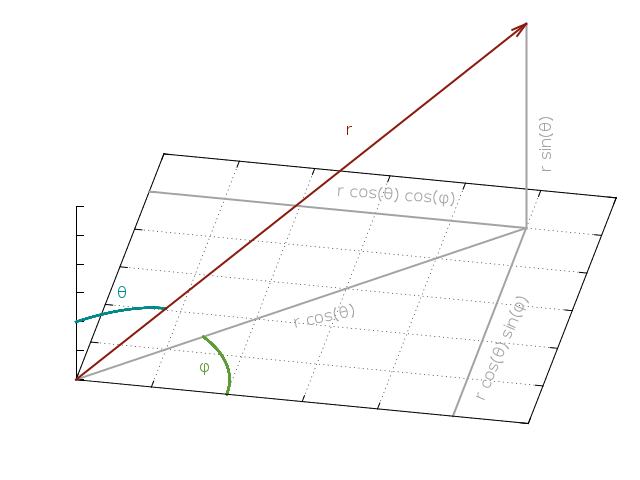
\includegraphics[scale=0.3]{SphericalCoordinates.png} 
		\end{center}
	\end{figure}
	
	 Pela Figura podemos ver que a posição é dada pelo vetor $\vec{r}$, onde:
	 \[ \vec{r} = r\hat{r} \]
	 \[ \vec{r} = r sin(\/theta) cos(\varphi) \hat{i} + r sin(\theta) sin(\varphi) \hat{j} + r cos(\theta) \hat{k} \]
	 de modo que $\hat{r}$:
	 \[ \hat{r} = sin(\theta) cos(\varphi) \hat{i} + sin(\theta) sin(\varphi) \hat{j} + cos(\theta) \hat{k} \]	
	 além disso temos:	
	 \[ \hat{\varphi} = \hat{k}\quad \text{x}\quad \hat{r}  = -sin(\varphi) \hat{i} + cos(\varphi) \hat{j}\]
	 \[ \hat{\theta} = \hat{\varphi}\quad  \text{x} \quad   \hat{r} = cos(\theta) cos(\varphi) \hat{i} + cos(\theta) sin(\varphi) \hat{j} -  sin(\theta) \hat{k}\]
	 \indent	Com os versores definidos podemos calcular a aceleração e a velocidade em coordenadas esféricas.
	 \[ \vec{v} = \frac{d \vec{r} }{dt} = \dot{\vec{r}} = \dot{r} \hat{r} + r\dot{\theta} \hat{\theta}+ ( r \dot{\varphi} sin(\theta) ) \hat{\varphi} \]
	 	
	\begin{eqnarray*}
	\vec{a} = \frac{ d^2 \vec{r} }{ dt^2 } = &+&( \ddot{\vec{r}}  - r \dot{\theta}^2 -r\dot{\varphi}^2 sin(\theta)^2 )\hat{r} \\ 
	&+&( r \ddot{\theta} + 2 \dot{r} \dot{\theta} -r\dot{\varphi}^2 sin(\theta) cos(\theta) )\hat{\theta} \\
	 &+& ( r \ddot{\varphi} sin(\theta) + 2\dot{r} \dot{\varphi} sin(\theta) + 2r\dot{\theta} \dot{\varphi} cos(\theta) ) \hat{\varphi} 
	\end{eqnarray*}
	
	 Vemos nas equações acima que alguns termos são reconhecíveis, como: \\
	 
 	$\dot{r}\hat{r}$  \indent  Velocidade radial: velocidade com que o objeto se aproxima ou se afasta da origem na direção radial.
 \begin{figure}[h]
		\begin{center}
			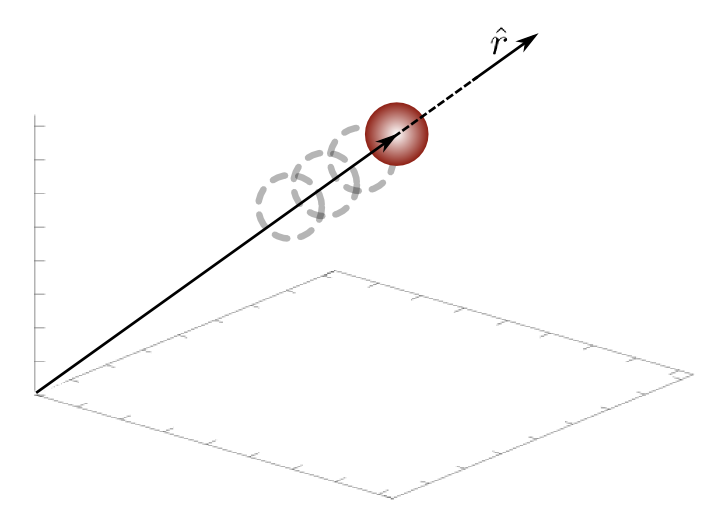
\includegraphics[scale=0.3]{SphericalCoordinatesMovR.png} 
			\caption{Movimento em $\hat{r}$}
		\end{center}
	\end{figure}
	
 $ r \dot{\theta}\hat{\theta}$ \indent Velocidade tangencial em $\theta$: é perpendicular a $\hat{r}$ sendo orientada na direção polar.
	\begin{figure}[h]
		\begin{center}
			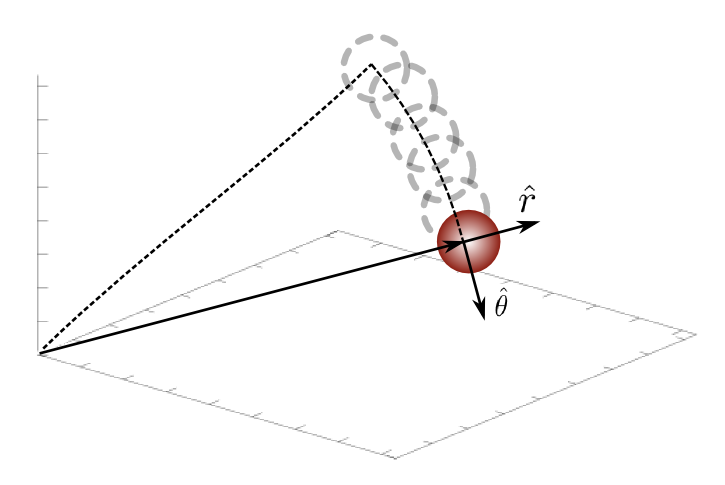
\includegraphics[scale=0.22]{SphericalCoordinatesMovTheta.png} 
			\caption{Movimento em $\hat{\theta}$}
		\end{center}
	\end{figure}
	\\ \\
	$rsin(\theta)\dot{\varphi}\hat{\varphi}$ \indent Velocidade tangencial em $\varphi$ : é perpendicular a $\hat{r}$ sendo orientada na direção azimutal.
	\begin{figure}[h]
		\begin{center}
			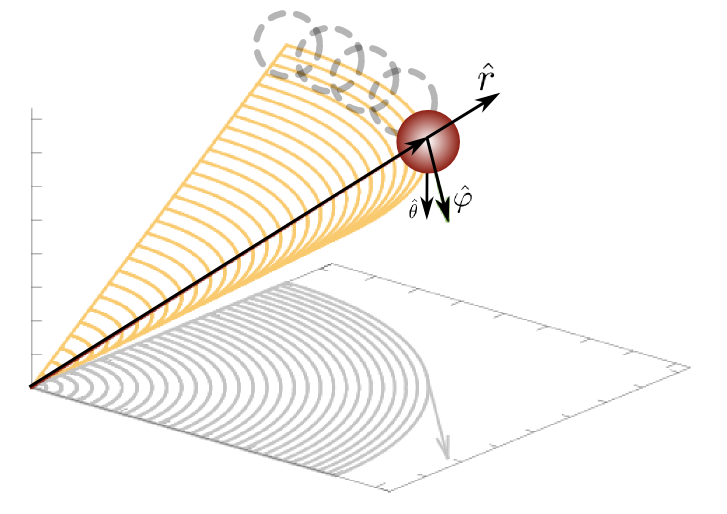
\includegraphics[scale=0.2]{SphericalCoordinatesMovPhi.png} 
			\caption{Movimento em $\hat{\varphi}$}
		\end{center}
	\end{figure}

	$\ddot{r} \dot{\theta}^2 r \hat{r} $ \indent Aceleração centripeta: Característico de movimentos curvilíneos ou circulares. Ela é perpendicular à velocidade e aponta para o centro da trajetória. 
	\begin{figure}[h]
		\begin{center}
			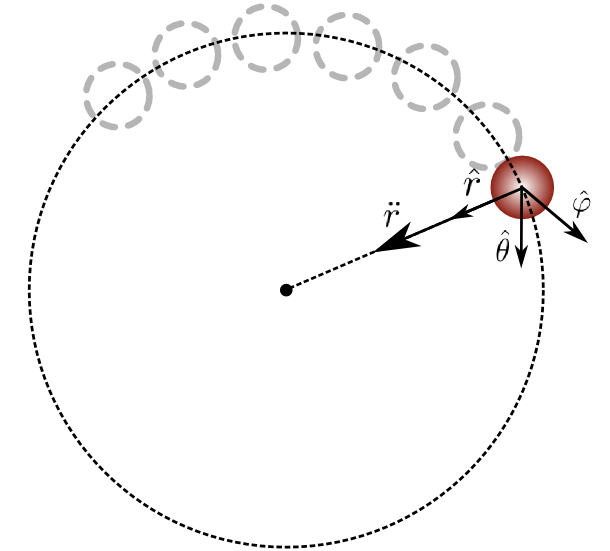
\includegraphics[scale=0.2]{SphericalCoordinatesDDOT_R.png} 
			\caption{Aceleração centripeta}
		\end{center}
	\end{figure}

	$ r \ddot{\theta} \hat{\theta} $\indent Aceleração angular: é a variação da velocidade angular no tempo
	\begin{figure}[h]
		\begin{center}
			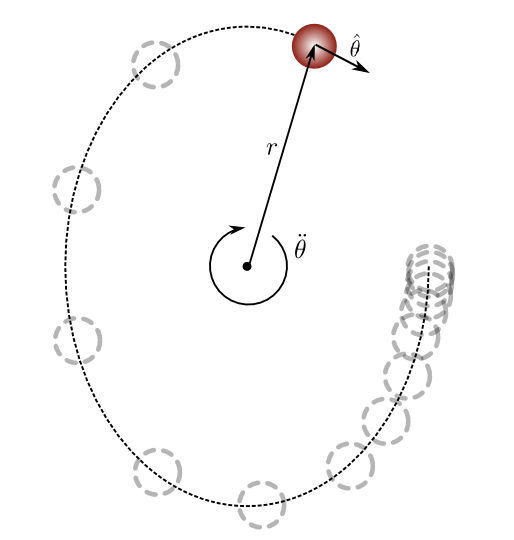
\includegraphics[scale=0.2]{SphericalCoordinatesDDOT_Theta.png} 
			\caption{Aceleração Angular}
		\end{center}
	\end{figure}

	$ 2\dot{r} \dot{\theta} \hat{\theta} \quad \text{e} \quad 2\dot{r}sin(\theta)\dot{\varphi}\hat{\varphi}$\indent Aceleração de Coriolis: Aceleração de um corpo que se move em relação a um sistema de referência, medida em outro sistema de referência que apresenta um movimento angular em relação ao primeiro.
\begin{figure}[h]
		\begin{center}
			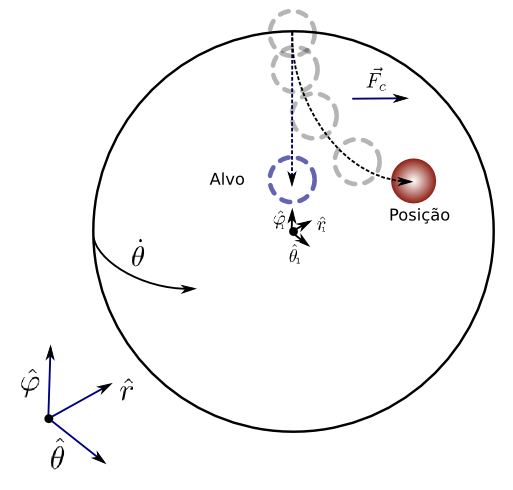
\includegraphics[scale=0.3]{SphericalCoordinatesCoriolis.png} 
			\caption{Efeito de Coriolis}
		\end{center}
	\end{figure}
	
	Na figura acima, o sistema de coordenadas $\hat{r_1}$,$\hat{\theta_1}$,$\hat{\varphi_1}$ esta em  movimento ($\dot\theta$ referencial inercial), a descrição do movimento no sistema $\hat{r}$,$\hat{\theta}$,$\hat{\varphi}$ (não-inercial) será diferente pois surgirá a força inercial provinda de $\dot\theta$
	
\end{document}

